% Baccalauréat malgache, série C, 2003 : corrigé.
\TCDBacAttribution{C}{2003}
\providecommand{\Plan}{(\mathscr{P})}
\providecommand{\dx}{\mathrm{d}x}
\providecommand{\Re}[1]{\mathrm{Re}\left( #1 \right)}
\providecommand{\Im}[1]{\mathrm{Im}\left( #1 \right)}
\providecommand{\dt}{\mathrm{d}t}
\providecommand{\Ouv}{(O;\vec{u},\vec{v})}
\providecommand{\mes}[2]{\mathrm{mes}\left( \widehat{ \overrightarrow{#1} ; \overrightarrow{#2} } \right)}
\providecommand{\D}{(\mathscr{D})}
\providecommand{\Courbe}{(\mathscr{C})}
\providecommand{\Courben}{(\mathscr{C}_n)}
\providecommand{\CourbeD}{(\mathscr{C}_2)}
\providecommand{\congru}[3]{#1 \equi #2 \quad \left[ \mathrm{mod}~#3\right]}
\providecommand{\Angl}[2]{\left( \widehat{ \overrightarrow{#1} , \overrightarrow{#2} } \right)}
\providecommand{\bary}[1]{\mathrm{Bar}\left\lbrace #1 \right\rbrace}
\providecommand{\Arg}[1]{\mathrm{Arg}\left( #1 \right)}
%
%%%%%%%%%%%%%%%%%%%%%%%%%%%%%%%%%%%%%%%%%%%%%%%%%%%%%%%%%%%%%%%%%%%%%%%%%%%%%%%%%%%%%%%%%%%%%%%%%%%%%%%%%%%%%%%%%%%%%%%%%%%%%%%%
\noindent \underline{\textsc{\textbf{Exercice}}} (4 points) 
\begin{description}
   \item[I. \textsc{Probabilit\'e}] ~\newline
      \begin{enumerate}
         \item \vln{Probabilit\'es de $A$ et $B$ :}
            Comme il y a 12 cas possibles :
            \begin{itemize}
               \item \ansbox{$P(A) = \frac{1}{12}$},
               \item $P(B) = \frac{3+4}{12}$ donc
                  \ansbox{$P(B) = \frac{7}{12}$}.
            \end{itemize}
         \item 
            \vln{Probabilit\'e de $C$ :}
            Pour totaliser 25 points, il faut avoir 10 + 10 + 5.
            Il y a $\frac{3!}{2! \ 1!} = 3$ moyens de le faire.
            $P(C) = \left( \frac{1}{12} \cdot \frac{1}{12} \cdot \frac{3}{12} \right) \cdot 3$.
            Ainsi, \ansbox{$P(C) = \frac{1}{192}$}.
                  
            \vln{Probabilit\'e de $D$ :}
            Pour totaliser un minimum de 21 points, on peut avoir : 
            \begin{itemize}
               \item 21 = 10 + 10 + 1, avec probabilit\'e
                  $\frac{1}{12}\cdot\frac{1}{12}\frac{4}{12}\cdot\frac{3!}{2!\cdot1!}$ ou
               \item 25 = 10 + 10 + 5, avec probabilit\'e 
                  $\frac{1}{12}\cdot\frac{1}{12}\cdot\frac{3}{12}\cdot\frac{3!}{2!\cdot1!}$ ou
               \item 30 = 10 + 10 + 10, avec probabilit\'e 
                  $\frac{1}{12}\cdot\frac{1}{12}\cdot\frac{1}{12}$.
            \end{itemize}
            Ainsi, $P(D) = \frac{1}{144} + \frac{1}{192} + \frac{1}{1728}$.
            D'o\`u \ansbox{$ P(D) = \frac{11}{864} $}.
      \end{enumerate}
   \item[II. \textsc{Arithm\'etique}]
      \begin{enumerate}
         \item \vln{Valeurs de $x^2$ pour $x\in\mathbb{Z}/6\mathbb{Z}$ :}
            \[
               \begin{array}{|c|c|c|c|c|c|c|}
               \hline 
               x & \bar{0} & \bar{1} & \bar{2} & \bar{3} & \bar{4} & \bar{5} \\ 
               \hline 
               x^2 & \bar{0} & \bar{1} & \bar{4} & \bar{9} & \bar{16} & \bar{25} \\ 
               \hline 
               \text{repr\'esentant} & \bar{0} & \bar{1} & \bar{4} & \bar{3} & \bar{4} & \bar{1} \\ 
               \hline 
               \end{array} 
            \]
            D'o\`u 
            $\displaystyle{
               \begin{array}{|c|c|c|c|c|c|c|}
               \hline 
               x & \bar{0} & \bar{1} & \bar{2} & \bar{3} & \bar{4} & \bar{5} \\ 
               \hline 
               x^2 & \bar{0} & \bar{1} & \bar{4} & \bar{3} & \bar{4} & \bar{1} \\ 
               \hline 
               \end{array} 
            }$
            en particulier, $x^2 \in \{ \bar{0} , \bar{1} , \bar{3} , \bar{4} \}$.
         \item \vln{Donn\'ee des quatre solutions de l'\'equation $x^p = x$ :}
            D'abord, on remarque que $\bar{0}^p = \bar{0}$ et $\bar{1}^p = \bar{1}$
            pour tout entier naturel non nul $p$.
            
            Notons aussi que $\bar{3}^2 = \bar{3}$ et que $\bar{4}^2 = \bar{4}$.
            Pour $x \in \{ \bar{3} , \bar{4} \}$, montrons par r\'ecurrence que $x^p = x$ :
            \begin{itemize}
               \item $x^1 = x$ est toujours vraie.
               \item \textbf{HR :} Supposons que $x^p = x$,
               \item On a alors $x^{p+1} = x^p \cdot x = x \cdot x = x$.
            \end{itemize}
            Donc les quatre solutions de $x^p = x$ sont \ansbox{$\bar{0}$, $\bar{1}$, $\bar{3}$ et $\bar{4}$}.
         \item \vln{Montrons que $x^3 = x$ pour tout $x \in \mathbb{Z}/6\mathbb{Z}$ :}
            On sait d'apr\`es la question pr\'ec\'edente que c'est vrai 
            pour $x \in \{ \bar{0} , \bar{1} , \bar{3} , \bar{4} \}$.
            De plus, 
            \begin{itemize}
               \item $\bar{2}^3 = \bar{4} \cdot \bar{2} = \bar{8} = \bar{2}$ et
               \item $\bar{5}^3 = \bar{1} \cdot \bar{5} = \bar{5}$,
            \end{itemize}
            On en d\'eduit
            \par\noindent\ansbox{$x^3=x$ pour tout $x\in\mathbb{Z}/6\mathbb{Z}$.}
         \item \vln{D\'eduisons que $n^3 - n$ est divisible par $6$ :}
            D'apr\`es la question pr\'ec\'edente, $x^3 = x$ pour tout $x \in \mathbb{Z}/6\mathbb{Z}$,
            ceci \'equivaut \`a $\congru{n^3}{n}{6}$ pour tout $n\in\mathbb{Z}$.
            Donc $\congru{n^3 - n}{0}{6}$. Par cons\'equent,
            \par\noindent\ansbox{$n^3-n$ est divisible par $6$ pour tout entier naturel $n$.}
      \end{enumerate}
\end{description}
%%%%%%%%%%%%%%%%%%%%%%%%%%%%%%%%%%%%%%%%%%%%%%%%%%%%%%%%%%%%%%%%%%%%%%%%%%%%%%%%%%%%%%%%%%%%%%%%%%%%%%%%%%%%%%%%%%%%%%%%%%%%%%%%
\noindent \underline{\textsc{\textbf{PROBLEME I}}} (7 points) \newline
Dans un plan orient\'e $\Plan$, soit $ABCD$ un carr\'e direct, de centre $J$.
\begin{description}
   \item[Partie A]~\newline
      \begin{description}
         \item[I. ]
            \begin{enumerate}
               \item \begin{enumerate}
									\item \vln{Nature et angle de $r'$ :}
										Comme $r'$ est la compos\'ee d'une translation et d'une rotation d'angle
										$\frac{\pi}{2}$, c'est une rotation d'angle $\frac{\pi}{2}$.
                        \item \vln{Images de $A$ et $B$ par $r'$ :}
									\begin{itemize}
										\item $r'(A) = t \left( r(A) \right) = t(A) = B$.
											Donc \ansbox{$r'(A) = B$}.
										\item $r'(B) = t \left( r(B) \right) = t(D) = C$.
											Donc \ansbox{$r'(B) = C$}.
									\end{itemize}
								\item \vln{D\'eduisons-en le centre de $r'$ :}
									Comme $r'(A) = B$,
									le centre de $r'$ se trouve sur la m\'ediatrice de $[AB]$.
									De m\^eme, $r'(B) = C$ alors le centre de $r'$ se trouve 
									sur la m\'ediatrice de $[BC]$.
									
										Le centre de $r'$ se trouve donc \`a l'intersection des deux m\'ediatrices.
										\par\noindent\ansbox{Le centre de $r'$ est $J$.}
							\end{enumerate}
					\item \begin{enumerate}
									\item \vln{Nature, angle et rapport de $f$ :}
										Comme $f$ est la compos\'ee d'une rotation d'angle $\frac{\pi}{2}$
										et d'une homoth\'etie de rapport $\sqrt{3}$, c'est une similitude directe
										d'angle $\frac{\pi}{2}$ et de rapport $\sqrt{3}$.
								\item \vln{Image de $C$ par $f$ :}
										Comme
										$f(C) = r' \left( h(C) \right) = r' (C) = D$, 
										alors \ansbox{$f(C) = D$}.
										
										\vln{Prouvons que $\Angl{IC}{ID} = \frac{\pi}{2}$ et $ID = \sqrt{3} IC$ :}
										Comme
										$\begin{multiform} f(I) = I \\ f(C) = D \end{multiform}$, alors
										$\Angl{IC}{ID} = \frac{\pi}{2}$ est \'egal \`a l'angle de $f$
										et $ID = k\, IC$ o\`u $k$ est le rapport de $f$.
										Ainsi,
										\ansbox{
										$
											\begin{multiform} 
												\Angl{IC}{ID} = \frac{\pi}{2} \\
												ID = \sqrt{3} IC .
											\end{multiform}
										$
										}
                        \item \vln{Donnons une mesure de l'angle $\Angl{CD}{CI}$ :}
                              Comme $\Angl{IC}{ID} = \frac{\pi}{2}$ alors 
                              $ICD$ est rectangle en $I$.
                              Il vient que 
                              $$\tan \Angl{CD}{CI} = \frac{ID}{IC} = \sqrt{3}.$$
                              On d\'eduit que 
                              \ansbox{$\Angl{CD}{CI} = \frac{\pi}{3}$}.
                                    
                              \vln{Pla\c{c}ons $I$ sur la figure :}
                              Plan de construction : 
                              \begin{itemize}
                                 \item tra\c{c}ons le cercle
                                    de centre $D$ et passant par $C$ puis
                                 \item tra\c{c}ons le cercle
                                    de centre $C$ et passant par $D$.
                                 \item Ces deux cercles se coupent en deux points $P$ et $P'$.
                                 \item Soient $Q$ et $Q'$ les milieux respectifs de 
                                    $[CP]$ et $[CP']$.
                                 \item On d\'eterminer lequel de $Q$ ou $Q'$ est le point $I$,
                                    pour cel\`a, on utilise le fait que 
                                    $\Angl{IC}{ID} = \frac{\pi}{2}$ (et non $-\frac{\pi}{2}$).
                                    \begin{figure}[h]
                                       \centering
                                       \begin{tikzpicture}[x=1.0cm,y=1.0cm]
                                          \draw [xstep=1.0cm,ystep=1.0cm, opacity=.2, line width=.2]
                                             (-2,-1) grid (10,9);
                                          \draw [xstep=0.5cm,ystep=0.5cm, opacity=.1, line width=.1]
                                             (-2,-1) grid (10,9);
                                          \draw [xstep=0.1cm,ystep=0.1cm, opacity=.05, line width=.05]
                                             (-2,-1) grid (10,9);
                                          \clip (-2,-1) rectangle (10,9);
                                          \fill[color=loko2,fill=loko2,fill opacity=0.1] 
                                             (0,4) -- (3,2.27) -- (4,4) -- cycle;
                                          \draw[thick,color=loko3b,fill=loko3b,fill opacity=0.1]
                                             (3.23,2.67) -- (2.83,2.91) -- (2.6,2.5) -- (3,2.27) -- cycle; 
                                          \draw [color=loko2!50!black, very thick] 
                                             (0,0)-- (4,0) -- (4,4) -- (0,4) -- cycle;
                                          \draw [color=loko5, very thin] (0,4) circle (4);
                                          \draw [color=loko5, very thin] (4,4) circle (4);
                                          \draw [color=loko2] (0,4)-- (3,2.27) -- (4,4) -- cycle;
                                          \fill [color=black] (0,0) circle (1.5pt) node[above right] {$A$};
                                          \fill [color=black] (4,0) circle (1.5pt) node[above right] {$B$};
                                          \fill [color=black] (4,4) circle (1.5pt) node[right] {$C$};
                                          \fill [color=black] (0,4) circle (1.5pt) node[above right] {$D$};
                                          \fill [color=black] (2,2) circle (1.5pt) node[above] {$J$};
                                          \fill [color=loko3] (2,0.54) circle (1.5pt) node[above] {$P$};
                                          \fill [color=loko3] (2,7.46) circle (1.5pt) node[above] {$P'$};
                                          \fill [color=black] (3,2.27) circle (1.5pt) node[below]
                                              {$\textcolor{loko3}{Q = }I$};
                                          \fill [color=loko3] (3,5.73) circle (1.5pt) node[below right] {$Q'$};
                                          \fill [color=loko1] (6,4) circle (1.5pt) node[below right] {$\Omega$};
                                          \draw [color=loko1, very thick] (6,4) circle (3.4641016151377544);
                                          \fill [color=loko1] (8,7) node [right] {$(E)$};
                                       \end{tikzpicture}
                                    \end{figure}
                              \end{itemize}
                           \item \vln{D\'eterminons $(E)$ :}
                                 Soient $\Omega = \bary{(D,1);(C,-3)}$ et 
                                 $\varphi$ la fonction scalaire de Leibniz associ\'ee au 
                                 syst\`eme $\{ (D,1);(C,-3) \}$.
                                 
                                  D\'eterminons $\Omega$ et $\varphi(\Omega)$ :
                                 \begin{align*}
                                    \overrightarrow{\Omega D} - 3\overrightarrow{\Omega C} & = \vec{0} \\
                                    \overrightarrow{\Omega D} - 3\overrightarrow{\Omega D} - 3\overrightarrow{DC}
                                          & = \vec{0} \\
                                    - 2\overrightarrow{\Omega D} & = 3\overrightarrow{DC} \\
                                    \overrightarrow{D\Omega} & = \frac{3}{2} \overrightarrow{DC} .
                                 \end{align*}

                                 Comme $\overrightarrow{\Omega D} - 3 \overrightarrow{\Omega C} = \vec{0}$, 
                                 $\overrightarrow{\Omega D} = 3 \overrightarrow{\Omega C}$ et donc 
                                 $\Omega D^2 = 9 \Omega C^2$.
                                 Par cons\'equent, 
                                 $\varphi(\Omega)=\Omega D^2-3\Omega C^2=9\Omega C^2-3\Omega C^2=6\Omega C^2$.

                                 Un point $M$ appartient \`a $(E)$ si : 
                                 \begin{align*}
                                    MD^2 - 3 MC^2 & = 0 \\
                                    -2 M\Omega^2 + \varphi (\Omega) & = 0 \\
                                    -2 M\Omega^2 + 6 \Omega C^2 & = 0 \\
                                    M\Omega^2 & = 3 \Omega C^2 \\
                                    M\Omega & = \sqrt{3} \Omega C .
                                 \end{align*}
                                 L'ensemble $(E)$ est donc le 
                                 cercle de centre $\Omega$ et de rayon $\sqrt{3} \Omega C$.
                                 %
                                 Remarquons que $I \in (E)$ ; 
                                 en effet, comme $ID = \sqrt{3} IC$ alors $ID^2 = 3\, IC^2$ et donc 
                                 $ID^2 - 3 \, IC^2 = 0$.
                                 %
                                 Finalement, en d\'eduit que 
                                 \ansbox{
                                 $(E)$ est le cercle de centre $\Omega$ et passant par $I$
                                 }.
                                 
                     \end{enumerate}
                  \end{enumerate}
               \item[II. ]
                  \begin{enumerate}
                     \item \vln{Affixes de $A$, $C$, $J$, $K$ :}
                        Pour un point $X$ quelconque, notons par $z_X$ son affixe.
                        On a 
                        \begin{itemize}
                           \item \ansbox{$z_A = 0$} car $A$ est l'origine.
                           \item \ansbox{$z_C = 1 + i$} car 
                              $\overrightarrow{AC}=1\cdot\overrightarrow{AB}+1\cdot\overrightarrow{AD}$.
                           \item \ansbox{$z_J = \frac{1}{2} + \frac{1}{2} i$} car 
                              $z_J = \frac{z_A + z_C}{2} = \frac{0 + 1 + i}{2}$.
                           \item \ansbox{$z_K = \frac{1}{2} + i$} car
                              $z_K = \frac{1 + i + i}{2}$.
                        \end{itemize}
                     \item \begin{enumerate}
                              \item \vln{Expression complexe de $S$ :}
                                 Soit $S : z' = az + b$ l'expression complexe de $S$.
                                 On sait que 
                                 $\begin{multiform} S(A) = J \\ S(C) = K \end{multiform}$ 
                                 donc 
                                 $\begin{multiform} z_J = a z_A + b \\ z_K = a z_C + b \end{multiform}$
                                 et 
                                 \begin{align*}
                                    a & = \frac{z_J - z_K}{z_A - z_C}      
                                        = \frac{(\frac{1}{2}+\frac{1}{2}i)-(\frac{1}{2}+i)}{(0)-(1+i)} 
                                        = \frac{-\frac{i}{2}}{-(1+i)}      \\
                                      & = \frac{\frac{i}{2} \cdot (1-i)}{(1+i)\; (1-i)}   
                                        = \frac{i + 1}{2 (1 + 1)}          
                                        = \frac{1}{4} + \frac{1}{4} i .
                                 \end{align*}
                                 Donc $b = z_J - a z_A = \frac{1}{2} + \frac{1}{2} i $.
                                 Ainsi, 
                                 \ansbox{$\displaystyle{
											S : z' = \left( \frac{1+i}{4} \right) \; z + \frac{1+i}{2}
                                 	}$}.
									\item \vln{\'El\'ements g\'eom\'etriques de $S$ : }
										\begin{itemize}
											\item Rapport : $k = \left| \frac{1+i}{4} \right| = \frac{\sqrt{2}}{4}$.
											\item Angle : 
												$\theta 
													= \Arg{\frac{1+i}{4}} 
													= \Arg{\frac{\sqrt{2}}{4} \; \left( \frac{\sqrt{2}}{2} + \frac{\sqrt{2}}{2} i \right)}
													= \frac{\pi}{4}$.
												Donc $\cos \theta = \frac{\sqrt{2}}{2}$ et $\sin \theta = \frac{\sqrt{2}}{2}$,
												ce qui donne $\theta = \frac{\pi}{4}$.
											\item Affixe du centre : 
												\begin{align*}
													z_\Omega 	& = \frac{\frac{1+i}{2}}{1-\frac{1+i}{4}}		
																  = \frac{\frac{1+i}{2}}{\frac{3-i}{4}}			
																  = \frac{2(1+i)(3+i)}{(3-i)(3+i)}				\\
																& = \frac{4+8i}{10}									
																  = \frac{2+4i}{5} .
												\end{align*}
											Ainsi, $S$ est la similitude plane directe de centre
											$\Omega\left(\frac{2}{5}+\frac{4}{5}i\right)$,
											de rapport $\frac{\sqrt{2}}{4}$ et d'angle $\frac{\pi}{4}$.
										\end{itemize}
                        \end{enumerate}
                  \end{enumerate}
         \end{description}
	\item[Partie B]~\newline
		\begin{enumerate}
			\item \vln{Nature de $R_E \circ R_F^{-1}$ :}
					Comme $R_E \circ R_F^{-1}$ est la compos\'ee de deux rotations dont la somme des angles est \'egale \`a $0$,
					$R_E\circ R_F^{-1}$ est une translation.
			\item \vln{D\'eduisons que $EHPQ$ est un parall\'elogramme :}
				Comme
				\begin{itemize}
					\item $R_E \circ R_F^{-1} (H) = R_E \left( R_F ^{-1} (H) \right) = R_E (E) = E$ et
					\item $R_E \circ R_F^{-1} (P) = R_E \left( R_F ^{-1} (P) \right) = R_E (G) = Q$, alors
				\end{itemize}
				\ansbox{$\overrightarrow{HE}=\overrightarrow{PQ}$ ; ce qui implique que $EHPQ$ est un parall\'elogramme.}
		\end{enumerate}
\end{description}
%%%%%%%%%%%%%%%%%%%%%%%%%%%%%%%%%%%%%%%%%%%%%%%%%%%%%%%%%%%%%%%%%%%%%%%%%%%%%%%%%%%%%%%%%%%%%%%%%%%%%%%%%%%%%%%%%%%%%%%%%%%%%%%%
\noindent \underline{\textsc{\textbf{PROBLEME II}}} (9 points)
\begin{description}
	\item[Partie A]
		\begin{enumerate}
			\item 
				\begin{enumerate}
					\item \vln{Etude du sens de variation de $g$ : }
						La fonction $g$ est d\'efinie et d\'erivable sur $]0 ; +\infty[$ avec 
						$g'(x) = \frac{1}{x^2} + \frac{1}{x} > 0 $ pour tout $x > 0$.
						Par cons\'equent, la fonction $g$ est croissante sur $]0;+\infty[$.
					\item \vln{Solution de l'\'equation $g(x)=0$ :}
							La fonction $g$ est continue et strictement croissante.
							De plus, $g\left(\frac{3}{2}\right) = \ln \frac{3}{2} - \frac{2}{3} < 0$
							et $g(2) = \ln 2 - \frac{1}{2} > 0$.
							On en d\'eduit que l'\'equation $g(x)=0$ admet une solution unique $\alpha$ telle que
							$\frac{3}{2}<\alpha<2$.
							
							\vln{Signe de $g(x)$ suivant les valeurs de $x$ :}
								Comme $g$ est croissante et qu'elle s'annule en $\alpha$ :
									\begin{itemize}
										\item $g(x) < 0$ pour tout $x \in ]0 ; \alpha[$,
										\item $g(\alpha) = 0$,
										\item $g(x) > 0$ pour tout $x \in ]\alpha ; +\infty[$.
									\end{itemize}
				\end{enumerate}
			\item \vln{Etude de la variation de $f$ :}
				La fonction $f$ est d\'efinie et d\'erivable sur $]0 ; +\infty[$ avec
				\begin{align*}
					f'(x) 	& = \frac{ \frac{1}{x} \expo{x} - \expo{x} \cdot \ln (x)}{(\expo{x})^2}			\\
							& = \frac{\frac{1}{x} - \ln x}{\expo{x}}												\\
							& = -\frac{g(x)}{\expo{x}}																	\;.
				\end{align*}
				Comme $\expo{x} > 0$ pour tout $x$, alors $f'(x)$ est de signe contraire \`a $g(x)$.
				Donc $f'$ est positive sur $]0 ; \alpha[$ et n\'egative sur $]\alpha ; +\infty[$.
				Ainsi,
					\begin{itemize}
						\item \ansbox{Sur $]0 ; \alpha[$ : $f$ est croissante,}
						\item \ansbox{Sur $[\alpha ; +\infty[$ : $f$ est d\'ecroissante}.
					\end{itemize}
			\item 
				\vln{Ecrire $f(\alpha)$ sans $\ln \alpha$ :}
					On sait que $g(\alpha) = 0$, c'est-\`a-dire $-\frac{1}{\alpha} + \ln \alpha = 0$, 
					ou encore $\ln \alpha = \frac{1}{\alpha}$.
					
						Il vient alors que
						\begin{align*}
						f(\alpha)
						  &= \frac{\ln \alpha}{\expo{\alpha}}
						   = \frac{1/\alpha}{\expo{\alpha}}
						   = \frac{1}{\alpha\expo{\alpha}}.
						\end{align*}
						\par\noindent\ansbox{$f(\alpha) = \dfrac{1}{\alpha\expo{\alpha}}$.}
					\vln{Encadrement de $f(\alpha)$ :}
						Nous allons montrer que
						\[
						\frac{\expo{-2}}{2}<f(\alpha)<\frac{2}{3}\expo{-\frac{3}{2}}.
						\]
					On sait que $\frac{3}{2} < \alpha < 2$ et donc, comme la fonction $\exp$ est croissante, 
					$\expo{\frac{3}{2}} < \expo{\alpha} < \expo{2}$.
					\[
					\begin{array}{rcccl}
					\frac{3}{2} 										& < & \alpha									& < & 2 							\\
					\expo{\frac{3}{2}} 							& < & \expo{\alpha} 						& < & \expo{2}			\\\hline
					\frac{3}{2} \expo{\frac{3}{2}}				& < & \alpha \expo{\alpha} 				& < & 2 \expo{2}				\\
					\frac{1}{\frac{3}{2} \expo{\frac{3}{2}}}& > & \frac{1}{\alpha \expo{\alpha}}	& > & \frac{1}{2 \expo{2}}	\\
					\frac{2}{3} \cdot \expo{-\frac{3}{2}}	& > & \frac{1}{\alpha \expo{\alpha}}	& > & \frac{1}{2} \expo{-2}	\\
					\frac{\expo{-2}}{2}							& < & \frac{1}{\alpha \expo{\alpha}}	& < & 2 \frac{\expo{-\frac{3}{2}}}{3}
					\end{array}
					\]
						d'o\`u
						\par\noindent\ansbox{
						$\displaystyle{\frac{\expo{-2}}{2}<f(\alpha)< 2 \frac{\expo{-\frac{3}{2}}}{3}}$
					}.
			\item \vln{Tra\c{c}age de $\Courbe$ :}
						\vln{Limites de $f$ aux bornes de son domaine de d\'efinition :}
							\begin{description}
									\item[En $0$ :] comme $\lim_{x\rightarrow 0^+}\ln x=-\infty$
										et $\lim_{x\rightarrow 0^+}\expo{x}=1$, alors
										\[
										\lim_{x\rightarrow 0^+}\frac{\ln x}{\expo{x}}=-\infty.
										\]
										L'axe des ordonn\'ees est donc asymptote verticale \`a la courbe $\Courbe$.
									\item[En $+\infty$ :]
										\[
										\lim_{x\rightarrow +\infty}\frac{\ln x}{\expo{x}}=0.
										\]
									L'axe des abscisses est donc asymptote horizontale de $\Courbe$ au voisinage de $+\infty$.
							\end{description}
						\vln{Tableau de variation de $f$ :}
							\begin{figure}[htb]
							\centering
							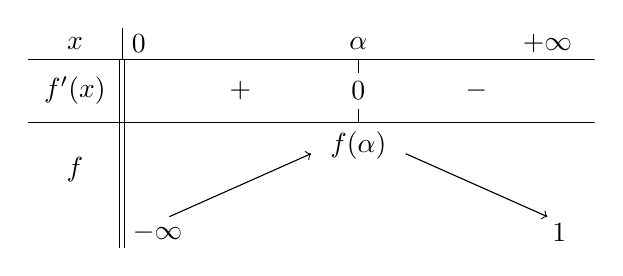
\begin{tikzpicture}[x=0.6cm,y=0.4cm]
								\clip(-6,-6) rectangle (6,1);
								\draw (-6,0)-- (6,0);
								\draw (-4,1)-- (-4,0);
								\draw (-3.95,0)-- (-3.95,-6);
								\draw (-4.05,0)-- (-4.05,-6);
								\draw (-6,-2)-- (6,-2);
								\draw (-5.,0.5) node[] {$x$};
								\draw (-5,-1) node[] {$f'(x)$};
								\draw (-5.,-3.5) node[ ] {$f$};
								\draw (-4,0.5) node[right] {$0$};
								\draw (5,0.5) node[ ] {$+\infty$};
								\draw (1,0.5) node[ ] {$\alpha$};
								\draw (1,0)-- (1,-2);
								\draw (1,-1) node[fill=white] {$0$};
								\draw (-1.5,-1) node[ ] {$+$};
								\draw (3.5,-1) node[ ] {$-$};
								\draw [->] (-3,-5) -- (0,-3);
								\draw [->] (2,-3) -- (5,-5);
								\draw (-3.25,-5.5) node[ ] {$-\infty$};
								\draw (5.25,-5.5) node[ ] {$1$};
								\draw (1,-2.75) node[ ] {$f(\alpha)$};
								\end{tikzpicture}
							\end{figure}
							%
							\begin{figure}
								\centering
								\begin{tikzpicture}[>=stealth,x=1.0cm,y=5.0cm]
								   \draw [xstep=1.0cm,ystep=1.0cm,opacity=0.2,line width=0.2] (-1.5,-2.5) grid (10,0.5);
								   \draw [xstep=0.5cm,ystep=0.5cm,opacity=0.1,line width=0.1] (-1.5,-2.5) grid (10,0.5);
								   \draw [xstep=0.1cm,ystep=0.1cm,opacity=.05,line width=.05] (-1.5,-2.5) grid (10,0.5);
								   \draw[->>] (-1.5,0) -- (10,0);
								   \foreach \x in {-1,1,2,3,4,5,6,7,8,9}
								   \draw[shift={(\x,0)}] (0pt,2pt) -- (0pt,-2pt) node[below] {\footnotesize $\x$};
								   \draw[<<->] (0,-2.5) -- (0,0.5);
								   \foreach \y in {-2.4,-2.2,-2,-1.8,-1.6,-1.4,-1.2,-1,-0.8,-0.6,-0.4,-0.2,0.2,0.4}
								   \draw[shift={(0,\y)}] (2pt,0pt) -- (-2pt,0pt) node[left] {\footnotesize $\y$};
								   \draw (0pt,-10pt) node[right] {\footnotesize $0$};
								   \draw [color=loko1](5,0.07) node[] {$(\mathscr{C})$};
								   \fill [] (1.76,0) circle (.5pt) node[below] {$\alpha$};
								   \fill [] (1.76,0.1) circle (.5pt);
								   \fill [] (0,0.1) circle (.5pt) node[left] {$f(\alpha)$};
								   \clip (-1.5,-2.5) rectangle (10,0.5);
									   \draw (0.5,0) node[above] {$\vec{\imath}$};
									   \draw (0,0.9) node[right] {$\vec{\jmath}$};
									   \draw [<->] (1.26,0.1) -- (2.26,0.1);
									   \draw [dashed] (0,0.1)-- (1.76,0.1);
									   \draw [dashed] (1.76,0.1)-- (1.76,0);
									   \draw [->,line width=1.2pt] (0,0) -- (1,0);
									   \draw [->,line width=1.2pt] (0,0) -- (0,1);
									   \draw[color=loko1, smooth,samples=100,domain=0.01:10.0] plot(\x,{ln((\x))*exp(-\x)});
								\end{tikzpicture}
							\end{figure}
							%
			\item \vln{Montrons que $G$ est d\'erivable :}
				Pour tout $x > 0$, la fonction $f$ est continue sur $[2x ; x^2]$ ou $[x^2 ; 2x]$ (selon les valeurs de $x$).
				De plus, les fonctions $x\mapsto 2x$ et $x\mapsto x^2$ sont d\'erivables pour tout $x > 0$.
				Par cons\'equent, \ansbox{$G$ est d\'erivable sur $]0 ; +\infty[$}.
				
				\vln{Calculons $G'(x)$ :}
				\[
					G'(x) 	= (x^2)' \cdot f(x^2) - (2x)' \cdot f(2x) = 2x \cdot \frac{\ln x^2}{\expo{x^2}} - 2 \cdot \frac{\ln 2x}{\expo{2x}}
				\]
				\ansbox{
					$\displaystyle{
						G'(x) = \frac{4 x \ln x}{\expo{x^2}} - \frac{2 \ln 2x}{\expo{2x}}
					}$
				}
		\end{enumerate}
	\item[Partie B]
		\begin{enumerate}
			\item \vln{\'Equivalence des \'equations $g(x)=0$ et $h(x)=x$ :}
					\begin{align*}
					g(x)=0
					&\iff -\frac{1}{x}+\ln x=0
					 \iff \ln x=\frac{1}{x}\\
					&\iff x=\expo{\frac{1}{x}}
					 \iff h(x)=x.
					\end{align*}
			\item \vln{Calcul de $h'(x)$ :}
				\ansbox{
					\[
						h'(x) = \left(\frac{1}{x}\right)' \cdot \expo{\frac{1}{x}} = -\frac{1}{x^2} \cdot \expo{\frac{1}{x}} .
					\]
					}
					
					\vln{V\'erifions que $\forall x \in \left[\frac{3}{2};2\right],\ 
							-\frac{4}{9}\cdot \expo{\frac{2}{3}} \leq h'(x) \leq -\frac{1}{4} \cdot \expo{\frac{1}{2}}$:}
						Soit $x\in \left[ \frac{3}{2} ; 2 \right]$, alors 
						\[
							\begin{array}{lll}
								\frac{3}{2} \leq x \leq 2 
									\Rightarrow & \frac{9}{4} \leq x^2 \leq 4 
										\Rightarrow & \frac{1}{4} \leq \frac{1}{x^2} \leq \frac{4}{9}
											\\
								\frac{3}{2} \leq x \leq 2 
									\Rightarrow & \frac{1}{2} \leq \frac{1}{x} \leq \frac{2}{3}
										\Rightarrow & \expo{\frac{1}{2}} \leq \expo{\frac{1}{x}} \leq \expo{\frac{2}{3}}
							\end{array}
						\]
						On multiplie membre-membre puis on inverse le signe :
						\[
							\frac{1}{4} \expo{\frac{1}{2}} 
								\leq \frac{1}{x^2} \expo{\frac{1}{x}} 
									\leq \frac{4}{9} \expo{\frac{2}{3}}
							\Rightarrow
							-\frac{4}{9} \expo{\frac{2}{3}}
								\leq -\frac{1}{x^2} \expo{\frac{1}{x}} 
									\leq -\frac{1}{4} \expo{\frac{1}{2}} .
						\]
				\vln{Existence d'un r\'eel $k\in]0;1[$ :}
						On sait que 
					$-\frac{4}{9} \expo{\frac{2}{3}} \leq h'(x) \leq -\frac{1}{4} \expo{\frac{1}{2}} \leq 0$,
						donc 
						$0 \leq |h'(x)| \leq \frac{4}{9} \expo{\frac{2}{3}} < 1$.
						Ainsi, on peut prendre $k = \frac{4}{9} \expo{\frac{2}{3}}$.
			\item \vln{Propri\'et\'e de contraction de $h$ :}
				On sait que $h$ est continue sur $\left[\frac{3}{2} ; 2 \right]$ 
				et d\'erivable sur $\left] \frac{3}{2} ; 2 \right[$.
				De plus, $|h'(x)| \leq k$ pour tout $x \in \left] \frac{3}{2} ; 2 \right[$.
					D'apr\`es le th\'eor\`eme des accroissements finis,
					\par\noindent\ansbox{Pour tous $x,y\in\left[\frac{3}{2};2\right]$,
					\newline $|h(x)-h(y)|\leq k|x-y|$.}
				\label{quest: Bac C 2003, pbm II, part B, 3/}
			\item 
				\begin{enumerate}
					\item \vln{Montrons que $\forall n \in \mathbb{N}$, $\frac{3}{2} \leq u_n \leq 2$ :}
						D\'emontrons cette propri\'et\'e par r\'ecurrence :
						\begin{itemize}
							\item Pour $n = 0$ : $\frac{3}{2} \leq u_0 = 2 \leq 2$. Donc la propri\'et\'e est vraie.
							\item Hypoth\`ese de r\'ecurrence : supposons que $\frac{3}{2} \leq u_n \leq 2$.
							\item Comme $h'(x) \leq 0$ alors la fonction $h$ est d\'ecroissante.
								Par cons\'equent 
								$ \frac{3}{2} \leq u_n \leq 2 \Rightarrow h \left( \frac{3}{2} \right) \geq h (u_n) \geq h(2)$,
								c'est-\`a-dire 
								$ \expo{\frac{2}{3}} \geq u_{n+1} \geq \expo{\frac{1}{2}} $.
								De plus, $2 \geq h(2) = \expo{\frac{2}{3}}$ et $h(2) = \expo{\frac{1}{2}} \geq \frac{3}{2}$ ;
								donc 
								\emph{$ \frac{3}{2} \leq u_{n+1} \leq 2$}.
								Ainsi, la propri\'et\'e est vraie \`a l'ordre $n+1$ et ceci ach\`eve notre d\'emonstration.
						\end{itemize}
						On d\'eduit que \ansbox{$\forall n \in \mathbb{N}$, $\frac{3}{2} \leq u_n \leq 2$.}
					\item \vln{Montrons que $\forall n \in \mathbb{N}$, $|u_{n+1}-\alpha|\leq k  |u_n-\alpha|$ :}
						Comme pour tout $n \in \mathbb{N}$, $u_n$ et $\alpha$ appartiennent \`a $\left[\frac{3}{2} ; 2 \right]$, 
						on peut appliquer le r\'esultat de la question~\ref{quest: Bac C 2003, pbm II, part B, 3/}
						en prenant $x = u_n$ et $y = \alpha$.
						On d\'eduit que \ansbox{$\forall n\in\mathbb{N}$, $|u_{n+1}-\alpha|\leq k  |u_n-\alpha|$.}
					\item 
						\vln{D\'eduction que $\forall n \in \mathbb{N}$, $|u_n - \alpha| \leq k^n |u_0 - \alpha|$ :}
							Utilisons l'in\'egalit\'e pr\'ec\'edente en rempla\c{c}ant $n$ successivement par $0$, $1$, \ldots , $n-1$.
							On multiplie membre-membre puis on simplifie :
							\[
								\begin{matrix}
										\times
									\underline{
										\left\lbrace
											\begin{array}{ccc}
												| u_1 - \alpha |	& \leq 	& k 	\cdot	| u_0 		- \alpha	| 	\\
												| u_2 - \alpha |	& \leq 	& k 	\cdot	| u_1 		- \alpha	| 	\\
														\vdots			& \vdots	&		\vdots								\\
												| u_n - \alpha |	& \leq 	& k 	\cdot	| u_{n-1}- \alpha	| 	
											\end{array}
										\right.
									}
									\\
										\quad \ 
										\begin{array}{rcl}
											| u_n - \alpha |	& \leq 	& k^n \cdot	| u_0 		- \alpha	| 	
										\end{array}
								\end{matrix}
							\]
							Ainsi, \ansbox{$\forall n \in \mathbb{N}$, $|u_n - \alpha| \leq k^n |u_0 - \alpha|$.}
							
						\vln{Calcul de la limite de $(u_n)$ :}
							Comme $0 \leq k < 1$, alors $\displaystyle{\lim_{n\rightarrow+\infty} k^n = 0}$.
							De plus, 
							\[
								\begin{array}{c}
									0 \leq |u_n - \alpha | \leq k^n \cdot |u_0 - \alpha |	\\
									\Downarrow	\\
									0 \leq \displaystyle{ \lim_{n\rightarrow +\infty} |u_n - \alpha | }
										\leq \displaystyle{ \lim_{n\rightarrow +\infty} k^n \cdot |u_0 - \alpha | }
										= 0 .
								\end{array}
							\]
							On d\'eduit que $\displaystyle{\lim_{n\rightarrow +\infty} |u_n - \alpha |}=0$ et donc que
							\ansbox{$\displaystyle{\lim_{n\rightarrow +\infty} u_n = \alpha}$}.
				\end{enumerate}
		\end{enumerate}
	\item[Partie C]
		\begin{enumerate}
			\item \vln{V\'erification que la fonction $f$ de la partie $A$ est solution de $(E)$ :}
				On sait d\'ej\`a que $f(x) = \frac{\ln x}{\expo{x}}$, $f'(x) = \frac{\frac{1}{x} - \ln x}{\expo{x}}$.
				Posons $u(x) = \frac{1}{x} - \ln x$ et $v(x) = \expo{x}$ ;
				on a $u'(x) = -\frac{1}{x^2} - \frac{1}{x}$ et $v'(x) = \expo{x}$.
				Il vient que 
				\begin{align*}
					f''(x) & = 
					\frac{\left( -\frac{1}{x^2} - \frac{1}{x} \right) \expo{x} - \expo{x} \left( \frac{1}{x} - \ln x \right)}
					{\left( \expo{x} \right)^2} \\
							& = \frac{-\frac{1}{x^2} - \frac{1}{x} - \frac{1}{x} + \ln x}{\expo{x}} = 
					\frac{\ln x - \frac{2}{x} - \frac{1}{x^2}}{\expo{x}} .
				\end{align*}
				On a alors 
				\begin{align*}
					f''(x) + 3 f'(x) + 2 f(x)
					& = \frac{\ln x - \frac{2}{x} - \frac{1}{x^2}}{\expo{x}} 
							+ 3 \frac{\frac{1}{x} - \ln x}{\expo{x}} 
							+ 2 \frac{\ln x}{\expo{x}} 																				\\
					& = \frac{\ln x-\frac{1}{x}-\frac{1}{x^2}+3\frac{1}{x}-3\ln x+2\ln x}{\expo{x}}					\\
					& = \frac{\frac{1}{x}-\frac{1}{x^2}}{\expo{x}} 															
					  = \frac{\frac{x-1}{x^2}}{\expo{x}} 																		
					  = \frac{x-1}{x^2} \cdot \expo{-x} .
				\end{align*}
				ce qui montre que $f$ est une solution de $(E)$.
			\item \vln{R\'esolution de $(E)$ :}
					Consid\'erons l'\'equation homog\`ene $(E_0) : y'' + 3y' + 2y = 0$.
					Elle a pour \'equation caract\'eristique $r^2 + 3 r + 2 = 0$.
				On a $\Delta = 3^2 - 4 \cdot 1 \cdot 2 = 1$ donc 
					$r_1 = \frac{-3-1}{2} = -2$ et $r_2 = \frac{-3+1}{2} = -1$.
				Ainsi, les solutions de $(E_0)$ sont de la forme $ A \expo{-2x} + B \expo{-x}$ o\`u $A$ et $B$ sont des r\'eels.
				
				L'ensemble des solutions de $(E)$ est donc
				\[
				\left\{
					x\mapsto A\expo{-2x}+B\expo{-x}+\frac{\ln x}{\expo{x}}
					\;\middle|\; (A,B)\in\mathbb{R}^2
				\right\}.
				\]
		\end{enumerate}
\end{description}
%%%%%%%%%%%%%%%%%%%%%%%%%%%%%%%%%%%%%%%%%%%%%%%%%%%%%%%%%%%%%%%%%%%%%%%%%%%%%%%%%%%%%%%%%%%%%%%%%%%%%%%%%%%%%%%%%%%%%%%%%%%%%%%%























